% !TEX root = ../master-thesis.tex

\begin{figure}[h!]
    \centering
    \addletter{85}{a} \phantom{4}
    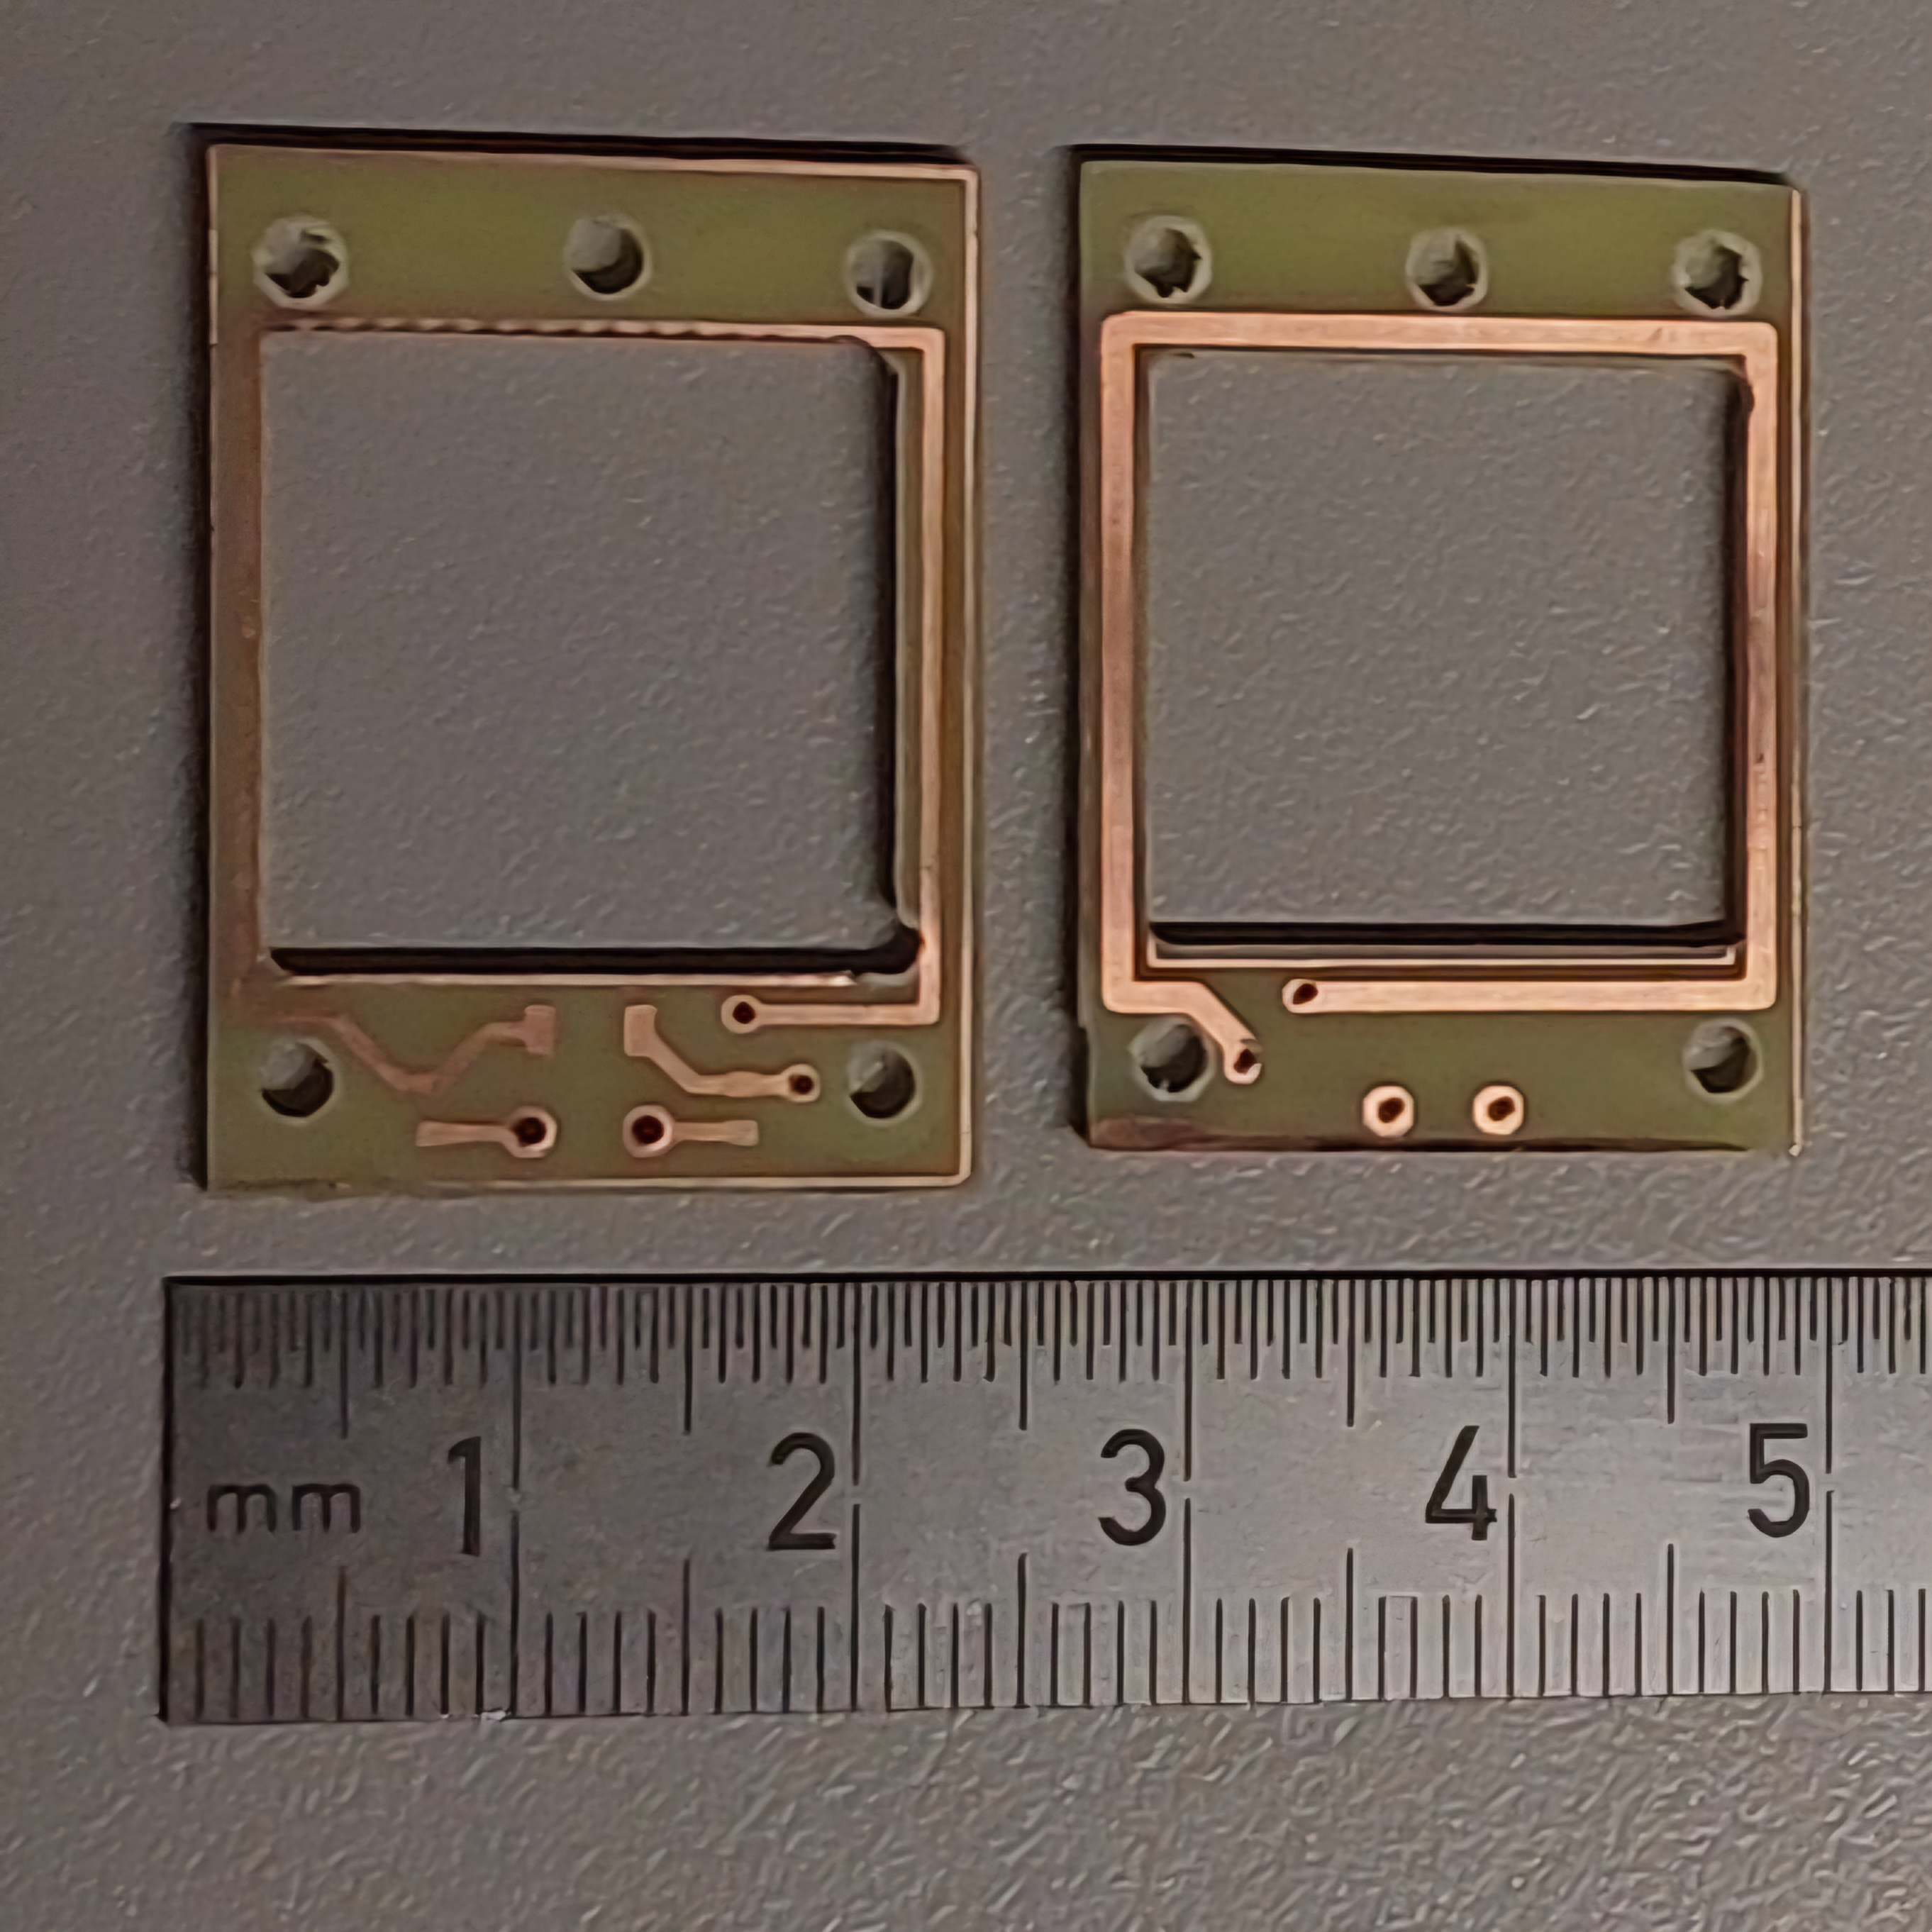
\includegraphics[width=1.25in]{imgs/RF.jpg}
    \hspace{1cm}
    \addletter{85}{b} \phantom{4}
    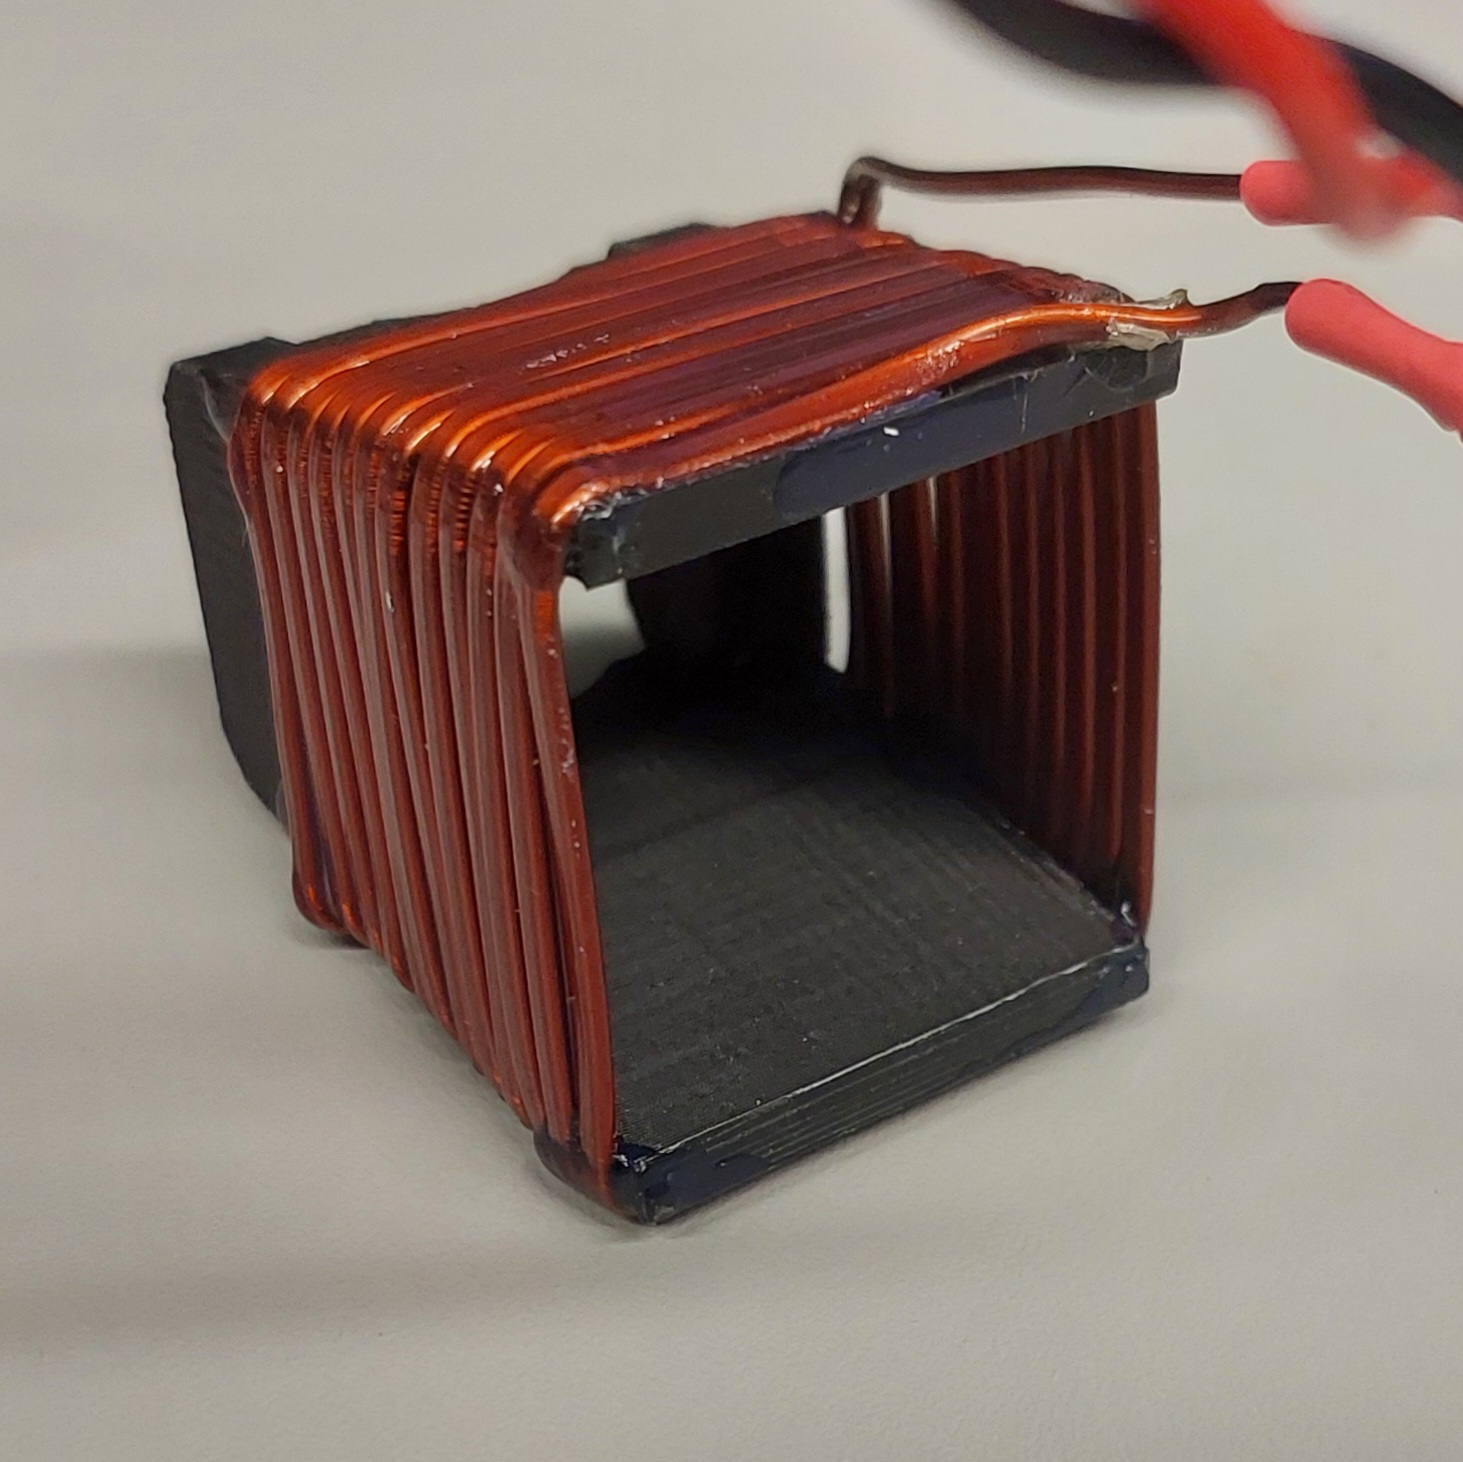
\includegraphics[width=1.25in]{imgs/MW.jpg}
    \caption{
        \textbf{RF and MW antennas used for spin control.}
        (a) PCB-based radiofrequency (RF) antenna used for driving spin transitions at MHz frequencies. 
        (b) Microwave (MW) loop antenna, designed to efficiently couple to hyperfine transitions in $^6$Li. 
        These antennas are used for coherent spin manipulation.
        % performance characterization via spin-flip fidelity is discussed in the following figures.
    }
    \label{fig:rfmw}
\end{figure}


\begin{figure}[h!]
    \centering
    \addletter{130}{a}
    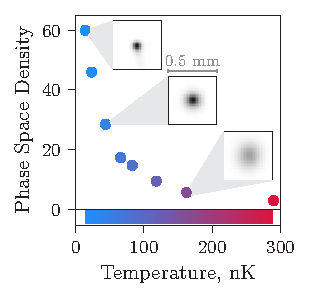
\includegraphics{fig-ai/m-bec-1-joined.pdf}
    \addletter{130}{b}
    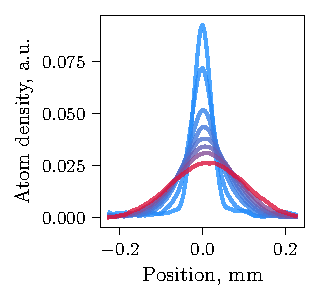
\includegraphics{fig-py/m-bec-2.pdf}
    \addletter{130}{c}
    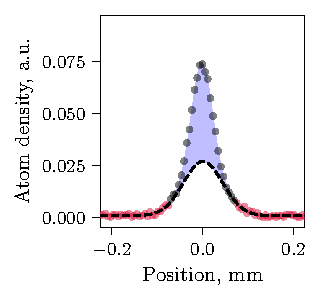
\includegraphics{fig-py/m-bec-3.pdf}
    \caption{
        \textbf{Molecular Bose-Einstein condensate data.}
        (a) Phase space density (PSD) increases as temperature decreases via evaporative cooling, indicating condensation onset. 
        (b) Atom density profiles normalized to unit area; color encodes temperature as in (a).
        (c) At low temperature, the profile shows a bimodal shape: a Gaussian fit to thermal wings (red dots) underestimates the central peak, revealing the mBEC component (blue area).
    }
    \label{fig:mbec}
\end{figure}




\begin{figure}[h!]
    \centering
    \addletter{145}{a}
    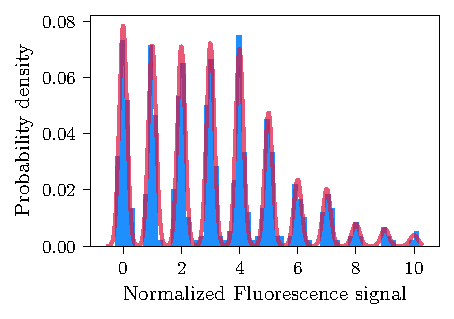
\includegraphics{fig-py/atom-counting.pdf}
    \phantom{4242}
    \addletter{145}{b}
    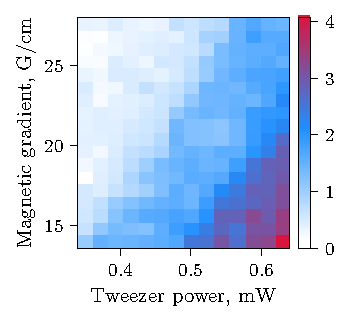
\includegraphics{fig-py/step-plot-2d.pdf}
    \caption{
        (a) Calibration histogram for single-atom counting based on fluorescence signal after after loading to the MOT. Clear quantized peaks correspond to integer atom numbers; the solid red line is a multi-Gaussian fit to the distribution. 
        (b) Measured 2D step plot as a function of tweezer power and magnetic field gradient. Each point indicates the average atom number obtained for a given combination of parameters. This map confirms that for any spill power, a suitable magnetic gradient can be found to achieve a desired quantized atom number.
    }
    \label{fig:spillingadd}
\end{figure}
